\documentclass{beamer}
% Replace the \documentclass declaration above
% with the following two lines to typeset your 
% lecture notes as a handout:
%\documentclass{article}
\usepackage{CJKutf8}
\usepackage[T1]{fontenc}
%\usepackage[utf8x]{inputenc}
\usepackage{graphicx}
\usepackage{subfigure}
\usepackage{mathtools}
\usepackage{ulem}
\usepackage{url}
\usepackage{pifont}
\usepackage{pgfplots}
\usepackage{textcomp}

\usepgfplotslibrary{external}
\pgfplotsset{width=10cm,compat=1.9}

\usetikzlibrary{shapes,arrows}

\tikzexternalize
\everymath{\displaystyle}

% There are many different themes available for Beamer. A comprehensive
% list with examples is given here:
% http://deic.uab.es/~iblanes/beamer_gallery/index_by_theme.html
% You can uncomment the themes below if you would like to use a different
% one:
%\usetheme{AnnArbor}
%\usetheme{Antibes}
%\usetheme{Bergen}
%\usetheme{Berkeley}
%\usetheme{Berlin}
%\usetheme{Boadilla}
%\usetheme{boxes}
%\usetheme{CambridgeUS}
%\usetheme{Copenhagen}
%\usetheme{Darmstadt}
%\usetheme{default}
%\usetheme{Frankfurt}
%\usetheme{Goettingen}
%\usetheme{Hannover}
%\usetheme{Ilmenau}
%\usetheme{JuanLesPins}
%\usetheme{Luebeck}
%\usetheme{Madrid}
%\usetheme{Malmoe}
%\usetheme{Marburg}
%\usetheme{Montpellier}
%\usetheme{PaloAlto}
%\usetheme{Pittsburgh}
%\usetheme{Rochester}
%\usetheme{Singapore}
%\usetheme{Szeged}
\usetheme{Warsaw}

\begin{document}
\begin{CJK}{UTF8}{gbsn}

\title{度假搜索系统结构的演变}

% A subtitle is optional and this may be deleted
\subtitle{2015年Q4晋级答辩}

\author{李庚\inst{1}}
% - Give the names in the same order as the appear in the paper.
% - Use the \inst{?} command only if the authors have different
%   affiliation.

\institute[Qunar.com] % (optional, but mostly needed)
{
  \inst{1}
  旅游度假事业部-搜索及频道 \\
  Qunar.com
}
% - Use the \inst command only if there are several affiliations.
% - Keep it simple, no one is interested in your street address.

\date{\today}

\AtBeginSection[]
{
  \begin{frame}<beamer>{纲要}
    \tableofcontents[currentsection,currentsubsection]
  \end{frame}
}

\begin{frame}
  \titlepage
\end{frame}

\begin{frame}{自我介绍}
  \begin{columns}
    \column{0.4\textwidth}
    \begin{itemize}
      \item { 李庚 }
      \item { 2010年7月毕业,同年入职 }
    \end{itemize}
    \column{0.6\textwidth}
    \begin{itemize}[1]
      \item<2-> 度假搜索系统技术Leader
      \item<3-> QTalk Code Contributor, Emacs版QTalk开发者与维护者
    \end{itemize}
  \end{columns}  
\end{frame}

\begin{frame}{自我介绍(续)}
  \begin{itemize}
  \item {度假搜索系统技术Leader \& 产品需求规划}
  \end{itemize}
  \vspace{3 mm}
  \begin{columns}
    \column{0.6\textwidth}
    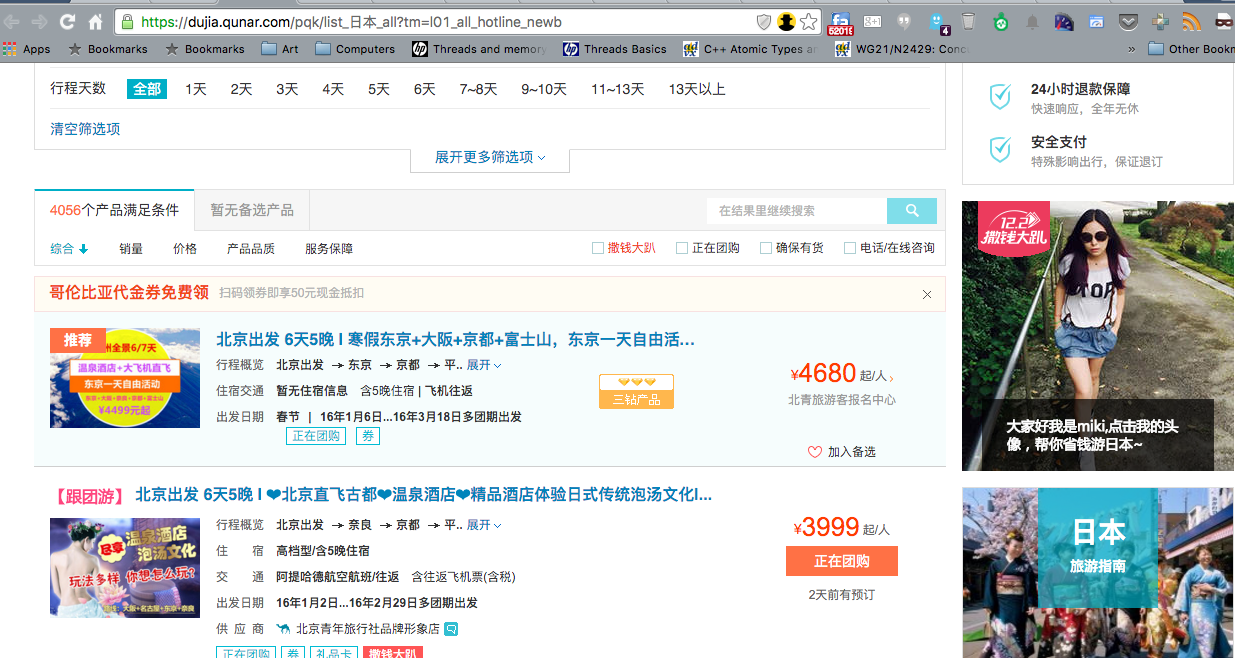
\includegraphics[scale=0.15]{./images/pc-search-screenshot}
    \column{0.4\textwidth}
    %% 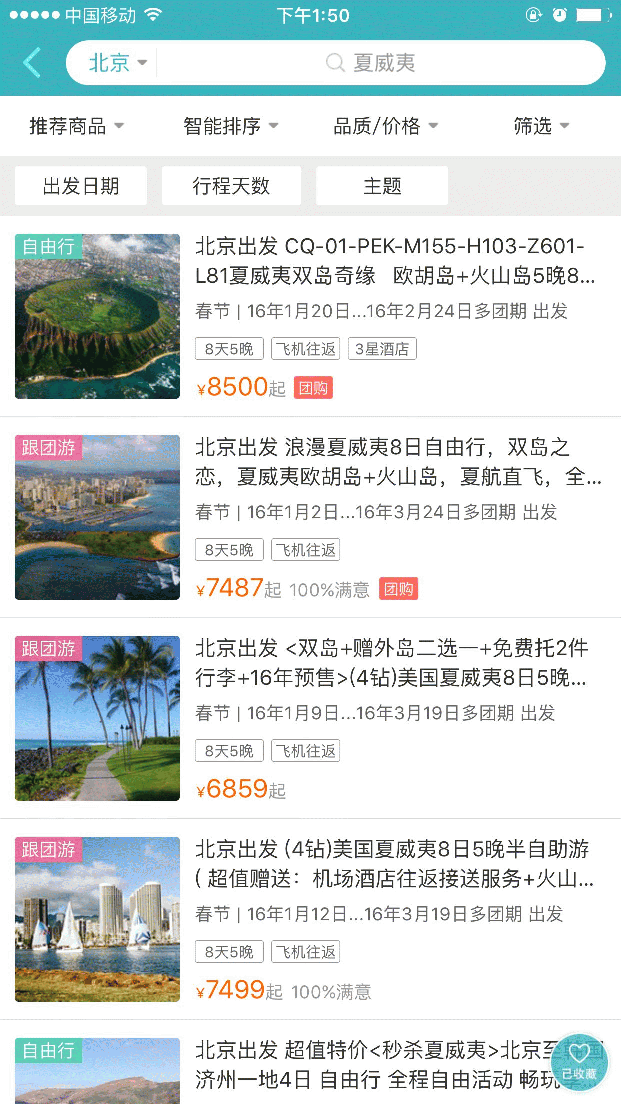
\includegraphics[scale=0.5]{./images/mobile-search-screenshot}
  \end{columns}
\end{frame}

\begin{frame}{自我介绍(续)}
  \begin{itemize}
  \item {QTalk Code Contributor, Emacs版QTalk开发者与维护者}
  \end{itemize}
  \begin{center}
    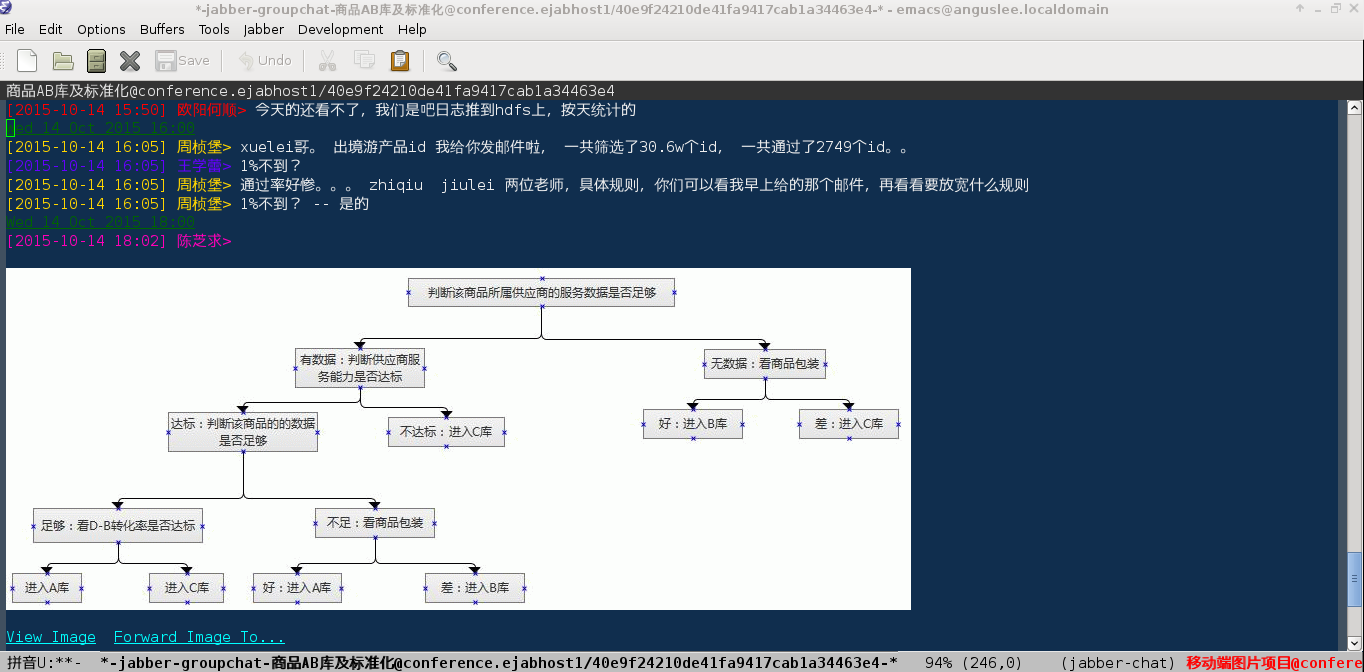
\includegraphics[scale=0.3]{./images/qtalk-emacs-screenshot}
  \end{center}
\end{frame}

\begin{frame}{纲要}
  \tableofcontents
\end{frame}

\section{搜索系统在业务中的定位}


\begin{frame}{事业部的目标}
  \begin{itemize}
  \item { 整合不同供应商提供的各类产品,满足用户的出行需求。
    \begin{itemize}
      \item<2-> { GMV: Gross Merchandise Value,总交易额 }
      \item<2-> { 毛利:$GMV - \text{成本} $ }
    \end{itemize}
  }
  \end{itemize}
\end{frame}

\begin{frame}{搜索团队要应对的问题}
  \begin{enumerate}
    \item { 随着业务量的膨胀,搜索服务的质量和效率不能降低 }
  \end{enumerate}
  \uncover<2-> {
    \begin{center}
      \begin{tikzpicture}[scale=0.75]
        \begin{axis}[
            title={产品规模随时间的演变趋势},
            xlabel={年份},
            ylabel={度假搜索覆盖的单品数量(万)},
            xmin=2012, xmax=2015,
            ymin=0, ymax=120,
            xtick={2012,2013,2014,2015},
            ytick={0,20,40,60,80,100,120},
            legend pos=north west,
            ymajorgrids=true,
            grid style=dashed,
          ]
          
          \addplot[
            color=blue,
            mark=square,
          ]
          coordinates {
            (2012,10)(2013,29.5)(2014,59.5)(2015,108.4)
          };
          \legend{旅游度假产品}
        \end{axis}
      \end{tikzpicture}
    \end{center}
  }
\end{frame}

\begin{frame}{搜索团队要应对的问题(续)}
  \begin{enumerate}\setcounter{enumi}{1}
  \item {
    应对不断变化的需求模式
    \begin{itemize}
      \item { 前期:PC为主 }
      \item { 目前:mobile为主 }
    \end{itemize}
  }
  \end{enumerate}
\end{frame}

\begin{frame}{搜索在度假整体业务中的位置}
  \begin{itemize}
  \item { $$ GMV = \sum_{i \in S}{(UV_i \times A_i \times R_i \times M_i)} $$ }
  \item { UV: 独立用户访问量 }
  \item { \color{blue}{ A: 服务可用率 } }
  \item { \color{blue}{ R: UV至订单转化率 } }
  \item { M: 平均用户交易额 }
  \item { S: 访问来源 }
  \end{itemize}
\end{frame}

\section{系统演变过程}

\begin{frame}{基本原则}
  \begin{enumerate}
  \item {
    量化目标
    \begin{itemize}
    \item<2-> { 产品需求:明确的量化指标和评测方法; }
    \item<2-> { 技术需求:制定监控目标,总结效果; }
    \end{itemize}
  }
  \item {
    重视系统结构的效率
    \begin{itemize}
    \item<3-> { 降低故障和线上bug出现的可能性,使得团队多数时间在处理重要且不紧急的工作; }
    \item<3-> { 总结合适的设计模式快速满足常见需求; }
    \end{itemize}
  }
  \item {
    测量结果,快速试错
  }
  \end{enumerate}
\end{frame}

\begin{frame}{搜索系统结构划分}
  \tikzset{%
    block/.style    = {draw, thick, rectangle, minimum height = 1em,
      minimum width = 1em},
    sum/.style      = {draw, circle, node distance = 2cm}, % Adder
    input/.style    = {coordinate}, % Input
    output/.style   = {coordinate} % Output
  }
  % Defining string as labels of certain blocks.
  \newcommand{\suma}{\Large$+$}
  \newcommand{\inte}{$\displaystyle \int$}
  \newcommand{\derv}{\huge$\frac{d}{dt}$}

  \begin{tikzpicture}[auto, thick, node distance=1cm, >=triangle 45, scale=0.75]
    \draw
	% Drawing the blocks of first filter :
	node at (0,0)[right=-3mm]{\Large \textopenbullet}
	node [input, name=input1] {} 
	node [sum, right of=input1] (suma1) {\suma}
	node [block, right of=suma1] (inte1) {\inte}
    node at (6.8,0)[block] (Q1) {\Large $Q_1$}
    node [block, below of=inte1] (ret1) {\Large$T_1$};
    % Joining blocks. 
    % Commands \draw with options like [->] must be written individually
	\draw[->](input1) -- node {$X(Z)$}(suma1);
 	\draw[->](suma1) -- node {} (inte1);
	\draw[->](inte1) -- node {} (Q1);
	\draw[->](ret1) -| node[near end]{} (suma1);
	% Adder
    \draw
	node at (5.4,-4) [sum, name=suma2] {\suma}
    % Second stage of filter 
	node at  (1,-6) [sum, name=suma3] {\suma}
	node [block, right of=suma3] (inte2) {\inte}
	node [sum, right of=inte2] (suma4) {\suma}
	node [block, right of=suma4] (inte3) {\inte}
	node [block, right of=inte3] (Q2) {\Large$Q_2$}
	node at (9,-8) [block, name=ret2] {\Large$T_2$}
    ;
	% Joining the blocks of second filter
	\draw[->] (suma3) -- node {} (inte2);
	\draw[->] (inte2) -- node {} (suma4);
	\draw[->] (suma4) -- node {} (inte3);
	\draw[->] (inte3) -- node {} (Q2);
	\draw[->] (ret2) -| (suma3);
	\draw[->] (ret2) -| (suma4);
    % Third stage of filter:
	% Defining nodes:
    \draw
	node at (11.5, 0) [sum, name=suma5]{\suma}
	node [output, right of=suma5]{}
	node [block, below of=suma5] (deriv1){\derv}
	node [output, right of=suma5] (sal2){}
    ;
	% Joining the blocks:
	\draw[->] (suma2) -| node {}(suma3);
	\draw[->] (Q1) -- (8,0) |- node {}(ret1);
	\draw[->] (8,0) |- (suma2);
	\draw[->] (5.4,0) -- (suma2);
	\draw[->] (Q1) -- node {}(suma5);
	\draw[->] (deriv1) -- node {}(suma5);
	\draw[->] (Q2) -| node {}(deriv1);
    \draw[<->] (ret2) -| node {}(deriv1);
    \draw[->] (suma5) -- node {$Y(Z)$}(sal2);
    % Drawing nodes with \textbullet
    \draw
	node at (8,0) {\textbullet} 
	node at (8,-2){\textbullet}
	node at (5.4,0){\textbullet}
    node at (5,-8){\textbullet}
    node at (11.5,-6){\textbullet}
    ;
	% Boxing and labelling noise shapers
	\draw [color=gray,thick](-0.5,-3) rectangle (9,1);
	\node at (-0.5,1) [above=5mm, right=0mm] {\textsc{first-order noise shaper}};
	\draw [color=gray,thick](-0.5,-9) rectangle (12.5,-5);
	\node at (-0.5,-9) [below=5mm, right=0mm] {\textsc{second-order noise shaper}};
  \end{tikzpicture}  
\end{frame}

\begin{frame}{搜索系统结构划分(续)}
  \begin{block}{对外服务端}
    \begin{itemize}
    \item { WEB与API }
    \item { 倒排索引 }
    \end{itemize}
  \end{block}
  \begin{block}{后台处理}
    \begin{itemize}
    \item { 数据预处理 }
    \item { 数据挖掘 }
    \end{itemize}
  \end{block}
\end{frame}

\section{经验总结}

\begin{frame}{产品的目的地如何获取?}
  PlaceHolder
\end{frame}


\end{CJK}
\end{document}
